\documentclass[12pt]{article}

\usepackage[utf8]{inputenc}
\usepackage[T1]{fontenc}
\usepackage{geometry}
\usepackage{graphicx} %figures
\usepackage{subfig} %subfigures
\usepackage{gensymb} %degree sign
\usepackage{amsmath} %math stuff
\usepackage{bm} %bold stuff
\usepackage[]{algorithm2e} %algorithms
\geometry{a4paper}

\title{\textbf{Part 9: Stochastic Gradient Descent}}

\begin{document}
\date{February 1, 2021}
\maketitle

We are going to go over a more light hearted topic, that of stochastic gradient descent (SGD). The basic idea is as follows, if we are solving an optimization problem where solving for the gradient is difficult, usually in the case of doing large matrix inverses, we should use SGD. This often happens because (i) the gradient is composed of that large matrix inverse or is otherwise computationally difficult (ii) the gradient is composed of randomly distributed parameters.

\section{Basic SGD}

We need something to compare SGD to, so we will solve the ordinary least squares method (OLS) problem.

\begin{align*}
\beta_{OLS} = (X^T X)^{-1} X^T Y
\end{align*}

Where $X$ will be a $N \times p$ matrix with $N=10^3$ and $p=10^2$ and $Y=X_1+U(-0.2,0.2)$. Of course this is not a hard problem for python to solve on most computers. However, we could imagine harder problems such as medical databases having many more data points $N$. We could also imagine $p$ being much larger for images (remember that a typical image might have $p=360\times 360$ pixels).

\vspace{5mm}

For SGD we do normal gradient descent, but when we calculate the gradient we only use a random selection of points $\{X,Y\}$. In the full gradient descent of the least squares problem the gradient is as follows:

\begin{align*}
f(\beta)=\Sigma_i^N (Y_i-\beta X_i^T)^2
\end{align*}

\begin{align*}
\nabla f(\beta) = \Sigma_i^N 2(Y_i-\beta X_i^T) X_i
\end{align*}

\vspace{5mm}

Which is the likelihood of the least squares problem, but for SGD we will only use $B$ random selections of $\{X,Y\}$. Therefore, for this application of SGD, we are using point (i), where the matrix $X$ is large. Note also that $\nabla f(\beta)$ is the gradient of the loss function, which can be used in a standard gradient descent update rule.
 
\begin{figure}[h]
\centering
\subfloat[][SGD Multiple Iterations]{\includegraphics[width=0.35\textwidth]{Post_9_fig1}}
\subfloat[][Error for OLS and SGD]{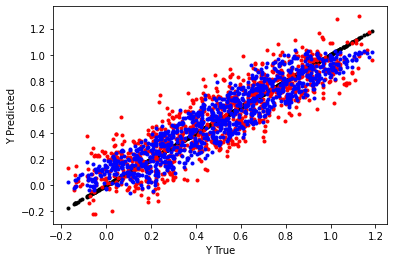
\includegraphics[width=0.35\textwidth]{Post_9_fig2}}
\caption{SGD for Solving Large Matrix Computation | blue = OLS, red = SGD}
\end{figure}

\vspace{5mm}

Here we will extend SGD to point (ii), where the problem is not large but itself stochastic. Let us have the same problem above except that $N=10^3$ and $p=10$ (a smaller problem) but let's assume the coefficients of the linear model are stochastically described by independent normal distributions.

\begin{align*}
\beta \sim N(\mu,I \times \sigma)
\end{align*}

\vspace{5mm}

Here we will use \textbf{all} data $\{X,Y\}$ when computing the likelihood $f(\beta)$, but we will do that process $B$ times using the above generating distribution. The trick to the update rule will be to have $\mu \approx \beta$ in the SGD loop. If you are confused look into the python code provided.

\begin{figure}[h]
\centering
\subfloat[][SGD Multiple Iterations]{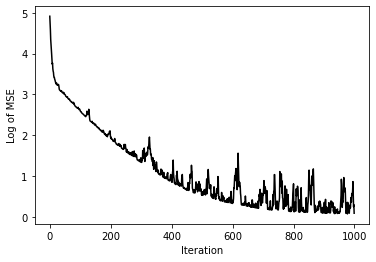
\includegraphics[width=0.35\textwidth]{Post_9_fig3}}
\subfloat[][Error for OLS and SGD]{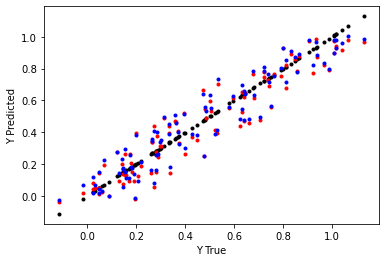
\includegraphics[width=0.35\textwidth]{Post_9_fig4}}
\caption{SGD for Solving Stochastic Parameter Problems | blue = OLS, red = SGD}
\end{figure}

\vspace{5mm}

This second problem, to me, seems much truer to form when it comes to SGD. We are literally calculating $\nabla f(\beta)$ $B$ times then taking an average, whereas in the first problem we aren't technically calculating the correct gradient to the deterministic problem. Either way we solve the problem efficiently.

\section{Advanced SGD}

Here we will discuss some more advanced versions of SGD, namely (i) ADAGRAD, (ii) RMSPROP, and (iii) ADAM. We will test all of them on the least squares problem with $N=100$ and $p=10$ for computational simplicity, but obviously such small problems could be solved with OLS.

\subsection{ADAGRAD}

The first advanced SGD is ADAGRAD, where we literally add the L2 norm of all previous gradient calculations for each parameter and divide the current gradient $\nabla f(\beta)$ by this weighting. This way larger parameters get dampened and those with smaller learning rates get artificially increased.

\begin{align*}
G_{jj} = \Sigma_t^T g_{t,j}^2
\end{align*}

\begin{align*}
\beta_j = \beta_j - \eta \dfrac{\nabla_j f(\beta)}{\sqrt{G_{jj}}}
\end{align*}

\vspace{5mm}

The result, as well as all results for advanced methods, is shown in Figure 2

\subsection{RMSPROP}

Next we have RMSPROP, or root-mean-squared propagation where we normalize the learning rate by a dampened L2 norm of the gradient. That dampened gradient is as follows:

\begin{align*}
v_{t+1} = \gamma v_{t}+(1-\gamma) (\nabla f(\beta))^2
\end{align*}

\vspace{5mm}

Now we take that dampened gradient and use that as a normalization factor for $\eta$.

\begin{align*}
\beta = \beta - \eta \dfrac{\nabla f(\beta)}{\sqrt{v}}
\end{align*}

\subsection{ADAM}

This last one is ADAM, or adaptive moment estimation. Here we take our gradient of the loss function $\nabla f(\beta)$ and modify it as such:

\begin{align*}
m = \alpha_1 m + (1-\alpha_1) \nabla f(\beta)
\end{align*}

\vspace{5mm}

Where $m$ acts as our new gradient modulated by a "forgetting factor" $\alpha_1$. We do the same with the square of the gradient:

\begin{align*}
v = \alpha_2 v + (1-\alpha_2) (\nabla f(\beta)^2)
\end{align*}

\vspace{5mm}

Which is the adjustment $v$ for the square of the loss gradient. We now calculate an effective gradient and squared loss gradient:

\begin{align*}
\hat{m}=\dfrac{m}{1-\alpha_1^{t+1}}
\end{align*}

\begin{align*}
\hat{v}=\dfrac{v}{1-\alpha_2^{t+1}}
\end{align*}

\vspace{5mm}

We get the update rule as such:

\begin{align*}
\beta = \beta + \eta \dfrac{\hat{m}}{\sqrt{\hat{v}}+\epsilon}
\end{align*}

\vspace{5mm}

Where $\epsilon=10^{-8}$, $\alpha_1=0.9$, and $\alpha_2=0.999$.

\begin{figure}[h]
\centering
\subfloat[][ADAGRAD]{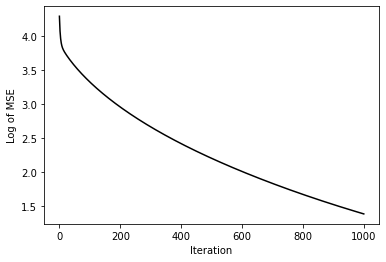
\includegraphics[width=0.35\textwidth]{Post_9_mse1}}
\subfloat[][RMSPROP]{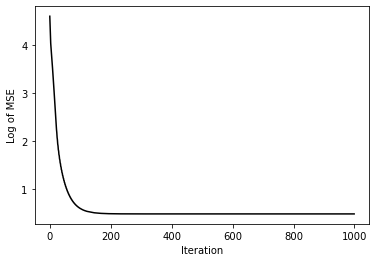
\includegraphics[width=0.35\textwidth]{Post_9_mse2}}
\subfloat[][ADAM]{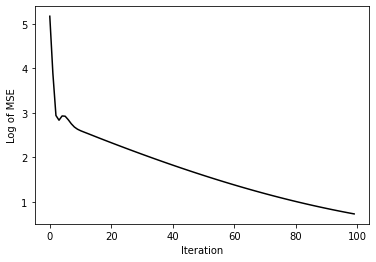
\includegraphics[width=0.35\textwidth]{Post_9_mse3}}

\subfloat[][ADAGRAD]{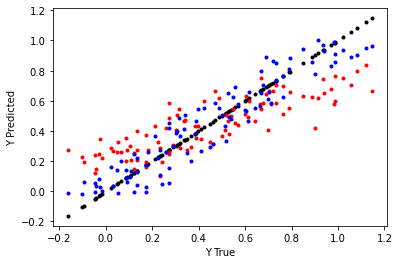
\includegraphics[width=0.35\textwidth]{Post_9_error1}}
\subfloat[][RMSPROP]{\includegraphics[width=0.35\textwidth]{Post_9_error2}}
\subfloat[][ADAM]{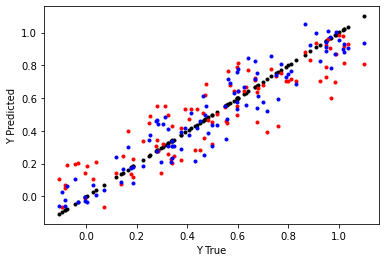
\includegraphics[width=0.35\textwidth]{Post_9_error3}}
\caption{Advanced SGD Algorithms | blue = OLS, red = SGD}
\end{figure}

\end{document}